\documentclass{article}
\usepackage[utf8]{inputenc}
\usepackage[spanish]{babel}
\usepackage{listings}
\usepackage{graphicx}
\graphicspath{ {images/} }
\usepackage{cite}

\usepackage[a4paper, lmargin=3cm, rmargin=3cm, bottom=2cm]{geometry}

\begin{document}

\begin{titlepage}
    \begin{center}
        
        
            
        \Huge
        \textbf{Nociones de la memoria del computador}
            
        \vspace{2.4cm}
        \LARGE
            
        \vspace{1.0cm}
        \LARGE
        \centering
        \textbf{Gabriel Antonio Lopera Madrid}\break
        \vspace{2cm}
        \LARGE
        \textbf{CC: 1020474048}\break
        \vspace{4cm}
        \LARGE
        \textbf{Informática 2}\break
        \vspace{1cm}
        \centering
       
        
\includegraphics[width=5cm]{udea.png} 
        
        \Large
        Despartamento de Ingeniería Electrónica y Telecomunicaciones\\
        Universidad de Antioquia\\
        Medellín\\
        Septiembre de 2020
            
    \end{center}
\end{titlepage}

\tableofcontents

\section{Introducción}
\noindent En informática, es importante conocer como es el funcionamiento real de un computador en su uso cotidiano, cuales procesos realiza y qué componentes hay de por medio para lograr todo lo que actualmente realizamos. La memoria o almacenamiento, corresponde con uno de los principales fines que tiene un computador en nuestro diario quehacer, sea en el ámbito educativo, laboral o recreativo, nos ayuda a procesar, retener y almacenar todos los diversos datos que para cada usuario diferente es importante. Existen distintos tipos de memorias, cada una cumple con su función determinada, tiene características y configuraciones específicas, que abordaremos de una manera resumida.

\section{¿Qué es la memoria de un computador?}
\noindent Es el dispositivo que cumple con una de las principales labores dentro del funcionamiento de un computador, el cual consta de memorizar, retener, o en otras palabras, almacenar datos por un periodo de tiempo determinado. De las diferentes memorias existentes, cada una cumple con su función específica pero con un fin común, el cual es generar una sincronización ideal para obtener un buen desempeño en el funcionamiento general del computador. \cite{gestion}

\section{Tipos de memorias conocidas} \label{contenido}

\subsection{Disco duro}

\noindent Es el dispositivo encargado de almacenar toda la información, programas y datos de un computador. Esta unidad es no volátil y hace parte de la memoria secundaria la cual quiere decir que no tiene acceso aleatorio y no pierde la información ante la ausencia de energía. Es el tipo de memoria que generalmente tiene la mayor capacidad de almacenamiento. Existen dos tipos de disco duro, HDD y SSD, siendo este último lo más reciente en discos duros, con mayor velocidad, mayor costo, pero menor capacidad de almacenamiento. \cite{wikipedia}

\begin{figure}[h]
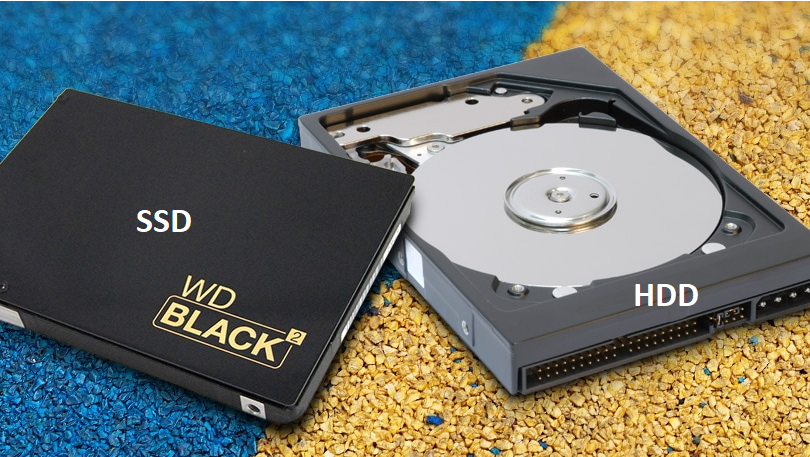
\includegraphics[width=4cm]{discoduro.PNG}
\centering
\caption{Disco duro SSD y HDD}
\end{figure}

\subsection{Memoria RAM}
\noindent Hace parte de la memoria principal del sistema, es volátil, es decir que pierde la información almacenada una vez se presente ausencia de la energía. Si bien es una de la memorias con menor capacidad de almacenamiento, dispone de una gran velocidad de lectura y escritura, y cumple así su función de recordar la información de los programas que se ejecutan en tiempo real en el computador, mejorando así el desempeño de la misma máquina. \cite{ram}
\begin{figure}[h]
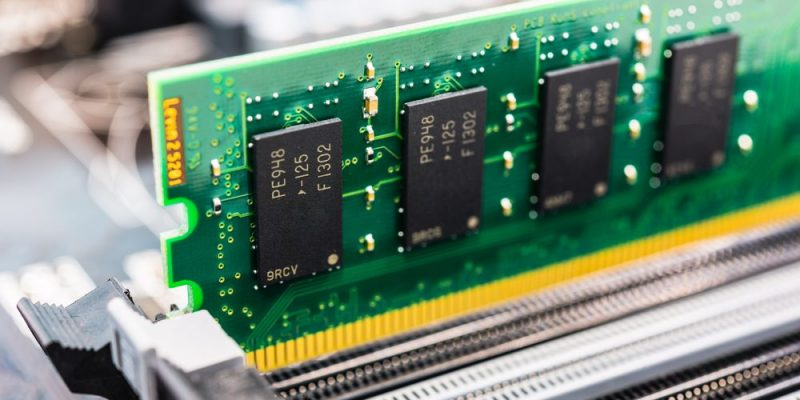
\includegraphics[width=4cm]{ram.jpg}
\centering
\caption{Memoria RAM}
\end{figure}

\subsection{Memoria virtual}
\noindent Es una técnica y configuración realizada en los dispositivos, que consta de acceder a una mayor parte de la memoria disponible, todo esto cuando la memoria RAM se llena, recurriendo así a utilizar una parte de memoria del disco duro. Gracias a esto, nuestro sistema puede usar parte del disco duro como si se tratara de memoria adicional, mejorando así la capacidad de procesamiento de nuestro computador. \cite{memoriavirtual}

\subsection{Memoria caché}
\noindent Es una memoria alterna que se sitúa entre el disco duro y la memoria RAM, siendo uno de los recursos del computador para almacenar datos que fueron recientemente procesados. Es tan eficaz que brinda tiempo extra al procesador accediendo de forma más rápido a diferentes datos, evitando así la búsqueda en el lugar de origen o disco duro.\cite{velocidad} \\

\vspace{1mm}

\noindent Actualmente se compone de 3 niveles establecidos en L1, L2 y L3, siendo este primero la más rápida de todas, aunque con una menor capacidad; El L2 consta de un equilibrio entre memoria y capacidad; Y por último se encuentra el L3 quien tiene una memoria mucho de más capacidad pero en menor velocidad de funcionamiento. Básicamente el funcionamiento integrado con el procesador es: la instrucción dada desde dicho procesador será buscada en la caché L1, si no encuentra información procede a la L2 y finalmente la caché L3. En caso de que no encuentre información continuará con la memoria RAM. 


\begin{figure}[h]
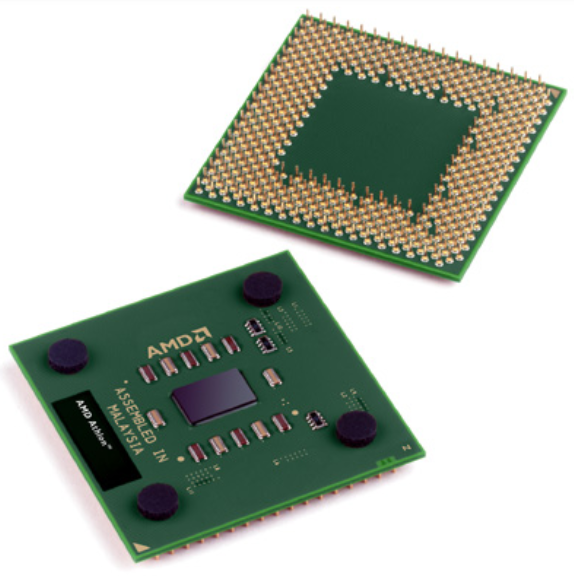
\includegraphics[width=4cm]{cache.PNG}
\centering
\caption{Memoria caché}
\end{figure}

\section{¿Cómo se gestiona la memoria de un computador?}
\noindent Mediante impulsos eléctricos viaja la orden enviada desde un periférico de entrada, esta consta de ir a buscar en un espacio de la memoria del disco duro el archivo a abrir. Luego es el microprocesador quien recibe la orden de ir a abrir ese espacio de la memoria encontrado el cual se encuentra en el disco duro. Para liberar memoria en el procesador, toda esta información se pasa a la memoria RAM que cuenta con más capacidad para trabajar y esta operación se repite millones de veces en sentidos contrarios cada vez que utilizamos el archivo. Asimismo, pasa cuando vamos a guardar alguna información, desde la memoria RAM se envía la instrucción el cual el microprocesador la lee y una vez recibida, va ejecutarla en el espacio de memoria del disco duro. Luego esta instrucción es eliminada tanto de la RAM como del microprocesador para liberar más espacio. \cite{gestion}

\vspace{5mm}

\section{¿Qué hace que una memoria sea más rápida que otra?}
\noindent La velocidad de una memoria, se ve afectada por la cantidad de megahercios que tenga cada una (MHz), entre mayor cantidad de MHz tenga la memoria, mayor será su velocidad, eso si, se reduce la capacidad de dicha memoria. Por eso generalmente la RAM que cuenta con menos capacidad, tiene una mayor velocidad que el disco duro, este último con una latencia más alta debido a la gran capacidad de almacenamiento. Esto es importante por el precio de las memorias, tener una memoria RAM de alta velocidad y gran capacidad, incrementa el costo exageradamente, cosa contraria al disco duro que puede ser barata a comparación de la gran capacidad que se puede tener. \cite{velocidad} \break
\vspace{1mm}

\noindent A continuación se observa una tabla comparativa entre la velocidad medida en MTs(horizontal) y CL(vertical), este último resulta del cálculo multiplicando el tiempo del ciclo del reloj, en nanosegundos, por el número de ciclos de reloj. Con esta gráfica se da una idea de tener un equilibrio entre estas dos medidas.

\begin{figure}[h]
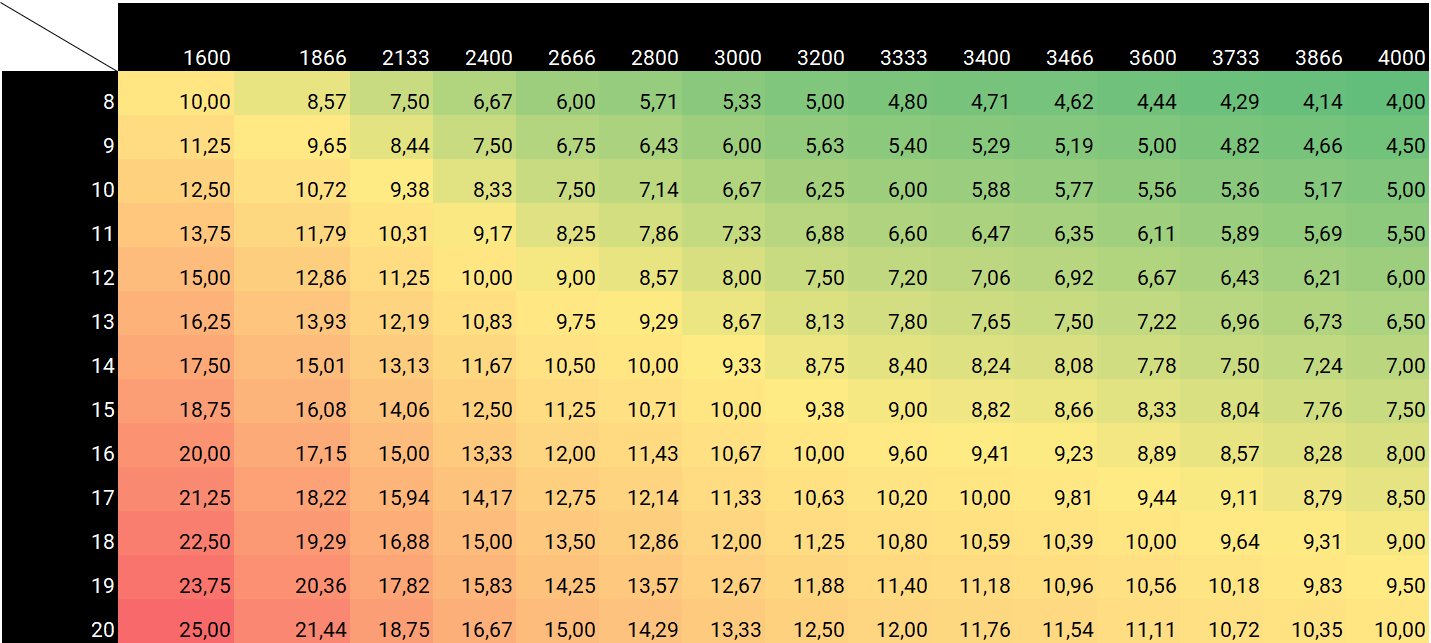
\includegraphics[width=12cm]{latencia.png}
\centering
\caption{Velocidad medida en Mts vs CL}
\end{figure}

\section{Conclusión} \label{conclulsion}
\noindent Se puede comprender de cierta manera como es la funcionalidad de un equipo y como influyen las diferentes memorias en ello, mejorando o afectando su rendimiento. Además, se observa y se logra entender con detalle, los motivos y finalidad de cada memoria, sea por mejorar la velocidad o reducir los costos de cada una de ellas.

\bibliographystyle{IEEEtran}
\bibliography{references}

\end{document}
